\documentclass{beamer}

% THEME SETTINGS
\usetheme{CambridgeUS}
\usecolortheme{dolphin}

% Bibliography
\usepackage[backend=biber, style=authoryear, citestyle=numeric]{biblatex}
\addbibresource{bibliography/bibliography.bib} % Point to your .bib file
\setbeamertemplate{frametitle continuation}{}


\title[SMOTE-DIRICHLET]{\LARGE SMOTE VARIANT FOR UNBALANCED DATA IN CLASSIFICATION PROBLEMS}
\author[De Stasio, Faccio, Suklan, Valentini]{\small Valeria De Stasio, Christian Faccio, Andrea Suklan, Agnese Valentini}

\begin{document}

% TITLE SLIDE
\begin{frame}
  \centering
  
\includegraphics[width=0.2\textwidth]{figures/logo.png} \\
  \rule{0.5\linewidth}{0.3pt}
  \titlepage
\end{frame}

% SLIDE 1
\begin{frame}
  \frametitle{Content}
  \begin{itemize}
    \item Introduction to the problem
    \item Data generation / Assessment method 
    \item SMOTE-DIRICHLET
    \item Results
  \end{itemize}
\end{frame}

%%%%%%%%%%%%%%%% Valeria %%%%%%%%%%%%%%%%%%%%%



%%%%%%%%%%%%%%%% Christian %%%%%%%%%%%%%%%%%%%%%

\section{Data Generation}

\begin{frame}
  \frametitle{Data Generation Process}
  
  \small
  \begin{table}[h]
    \centering
    \begin{tabular}{|c|c|c|}
    \hline
    Parameter & Values & Description \\ 
    \hline
    $n_\text{train}$ & 600, 1000, 5000 & Train set size \\  
    $n_\text{test}$ & 600 & Test set size \\
    $\pi$ & 0.10, 0.05, 0.025 & Proportion of rare examples \\
    $IR$ & 9, 19, 39 & Imbalance ratio \\
    \hline
    \end{tabular}
    \caption{Parameters of the simulation}
    \label{table:parameters}
    \end{table}


    \small
    \begin{equation*}
      (\mathbf{X}, y) \ \text{s.t.} \
      \begin{cases} 
          \mathbf{X} \sim N_2\left(
            \begin{pmatrix}
            0 \\ 0
            \end{pmatrix},
            \begin{pmatrix}
            1 & 0 \\ 
            0 & 1
            \end{pmatrix}
            \right) & \text{if } y = 0, \\
          \mathbf{X} \sim N_2\left(
            \begin{pmatrix}
            1 \\ 1
            \end{pmatrix},
            \begin{pmatrix}
            1 & -0.5 \\ 
            -0.5 & 1
            \end{pmatrix}
            \right) & \text{if } y = 1.
      \end{cases}
  \end{equation*}
\end{frame}

\begin{frame}
  \frametitle{Data Generation}
  \begin{figure}
    \centering
    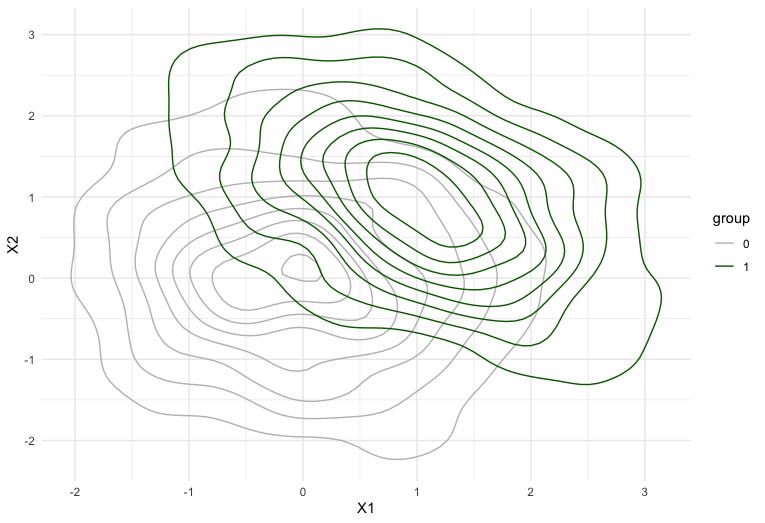
\includegraphics[width=0.8\textwidth]{figures/contour_data.png}
    \caption{Contour plot of the data distribution}
    \label{fig:contour_data}
  \end{figure}
\end{frame}

\begin{frame}
  \begin{figure}
    \centering
    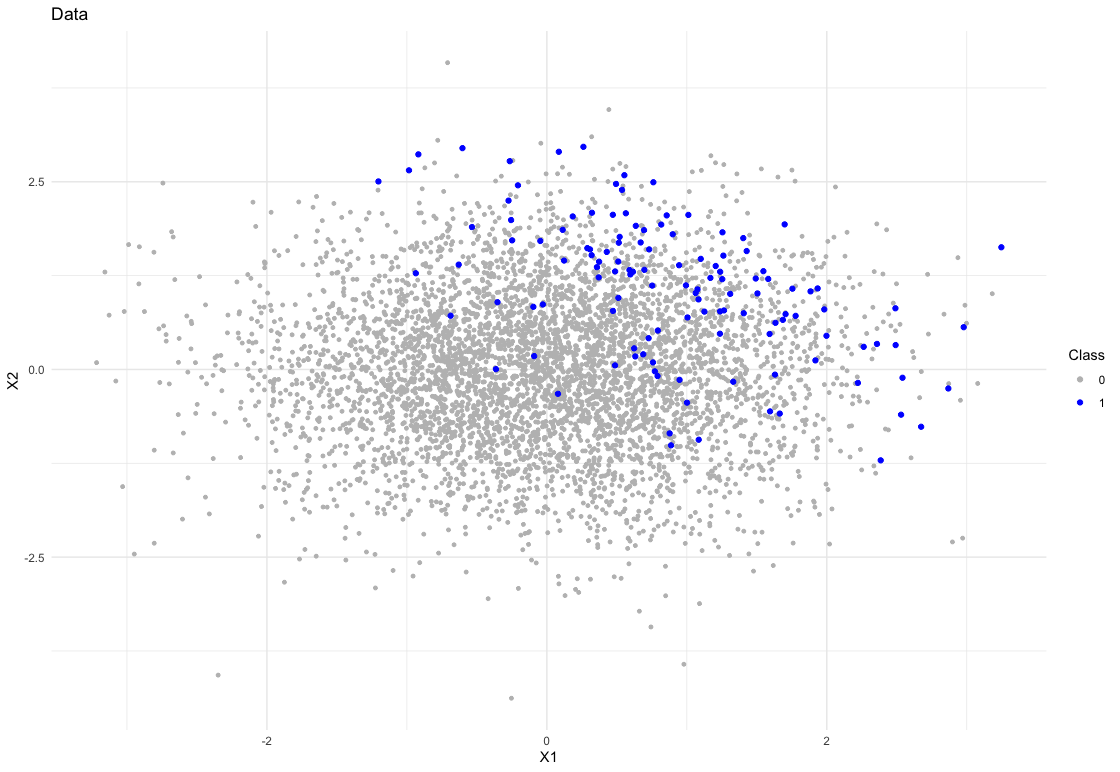
\includegraphics[width=0.8\textwidth]{figures/data.png}
    \caption{Data generated with $size = 5000$ and $prop = 0.025$}
    \label{fig:data}
  \end{figure}
\end{frame}


\begin{frame}
  \frametitle{Assessment Method}
  \begin{itemize}
    \item 100 Static Train/Test Division (test size = 600)
    \item Metrics: Balanced Accuracy, F1 Score
    \item Models: Decision Tree, Logistic Regression
    \item Comparisons with Boxplots
  \end{itemize}
\end{frame}





%%%%%%%%%%%%%%%% Agnese %%%%%%%%%%%%%%%%%%%%%


% AGNESE 

\begin{frame}{SMOTE}
  \begin{figure}
      \centering
      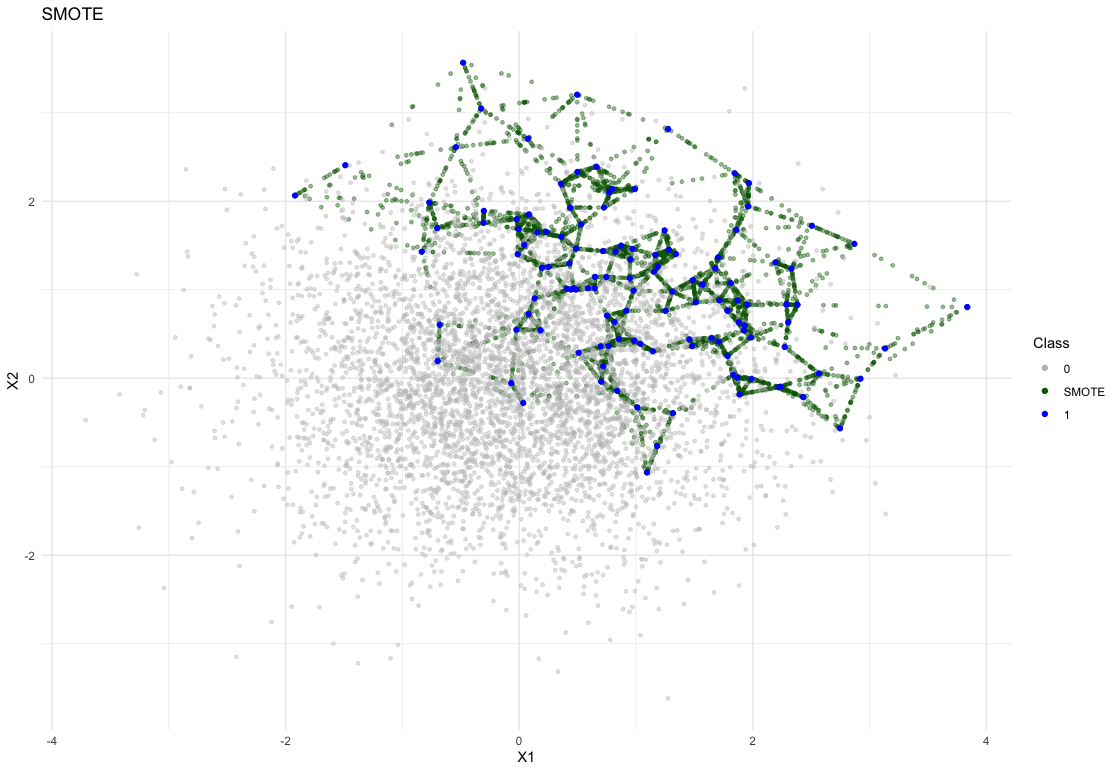
\includegraphics[width=0.8\linewidth]{figures/smote.png}
      \caption{Synthetic data generated with SMOTE}
      \label{fig:label1}
  \end{figure}
\end{frame}



\begin{frame}{Dirichlet SMOTE}
  \begin{figure}
      \centering
      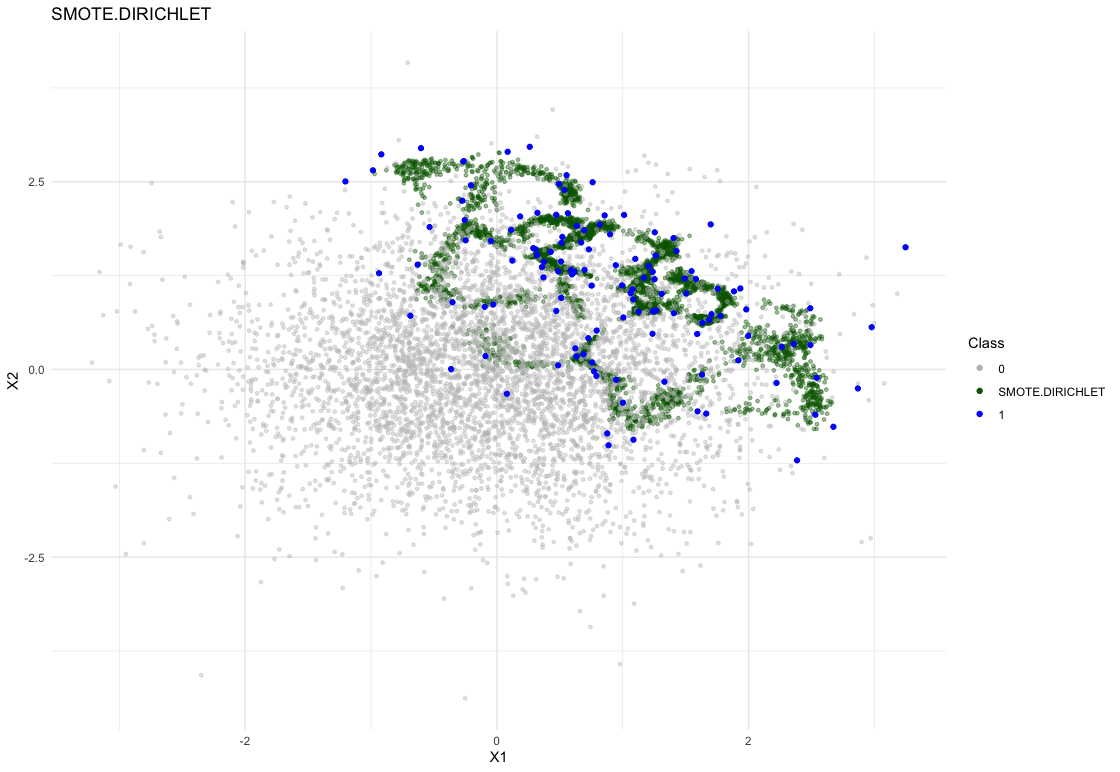
\includegraphics[width=0.7\linewidth]{figures/dirichlet.png}
      \caption{Synthetic data generated with Dirichlet SMOTE using Dirichlet distribution: $P(p|\alpha) \sim Dir(\alpha_1, ... , \alpha_k) = \frac{\Gamma(\sum_j \alpha_j )}{\Pi_j \Gamma(\alpha_j)} \Pi_{j = 1}^{k} p_j^{\alpha_j -1}$ \cite{matharaarachchi2024enhancing}. $\alpha = 1$, $k = 3,5$.}
      \label{fig:label2}
  \end{figure}    
\end{frame}




\begin{frame}{Comparison between SMOTE and Dirichlet SMOTE}
\begin{figure}
  \centering
  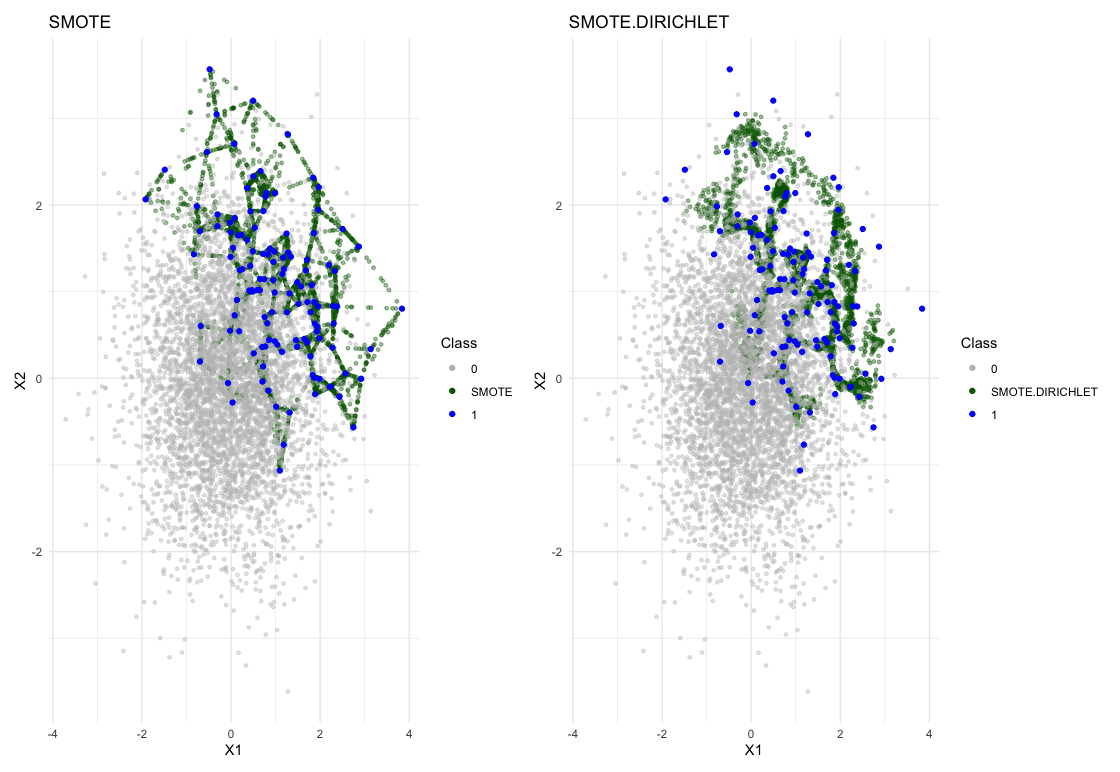
\includegraphics[width=1.03\linewidth, height = 6.5cm]{figures/combined.png}
  \label{fig:label3}
\end{figure}   
\end{frame}



%%%%%%%%%%%%%%%% Andrea %%%%%%%%%%%%%%%%%%%%%








%%%%%%%%%%%%%%%% REFERENCES %%%%%%%%%%%%%%%%%

\begin{frame}[allowframebreaks, plain]
  \frametitle{References}
  \nocite{*}
  \printbibliography
\end{frame}

\end{document}
